% \begin{figure}
%     \centering
%     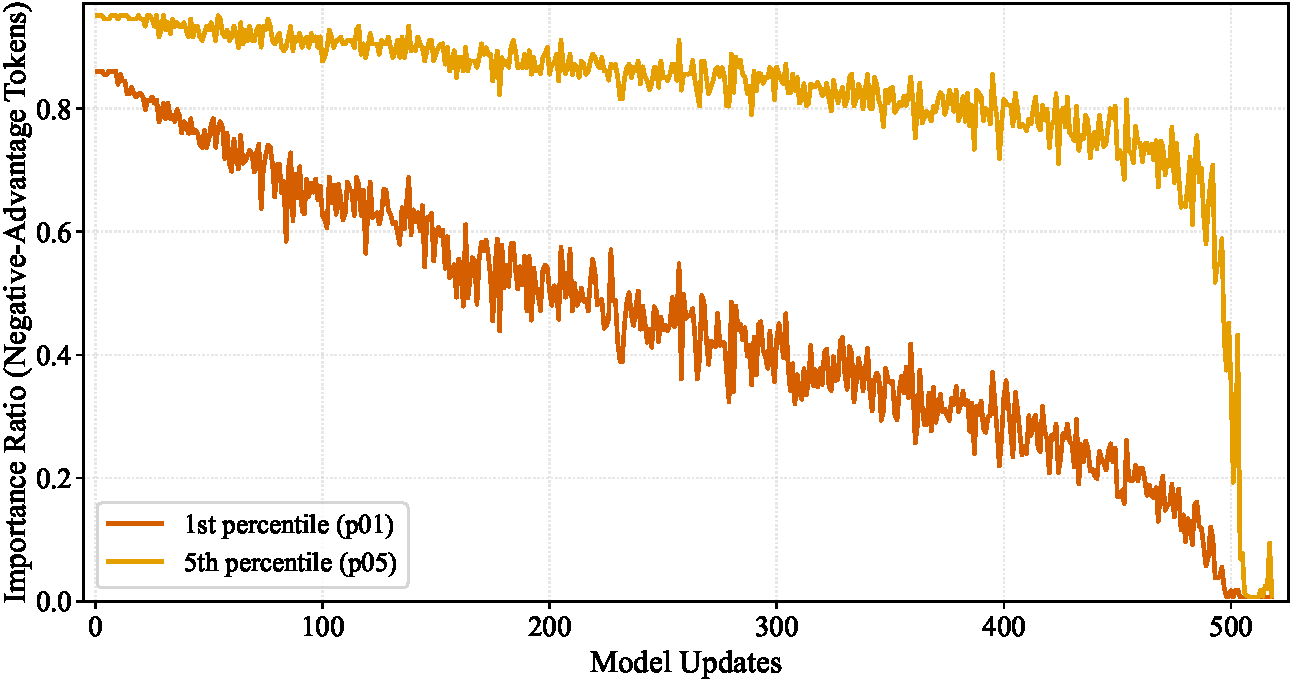
\includegraphics[width=0.4\textwidth]{figures/veto1.pdf}
%     \caption{Quantile evolution (p01 and p05) of importance ratios for negative-advantage tokens under high staleness.
% Lower quantiles drift steadily toward zero over training, revealing a systematic left-tail expansion of the distribution rather than isolated outliers.
% This degeneration precedes and anticipates the subsequent collapse in global training stability.}
%     \label{fig:veto1}
% \end{figure}
\begin{figure}[!h]
    \centering
    \begin{subfigure}[t]{0.48\textwidth}
        \centering
        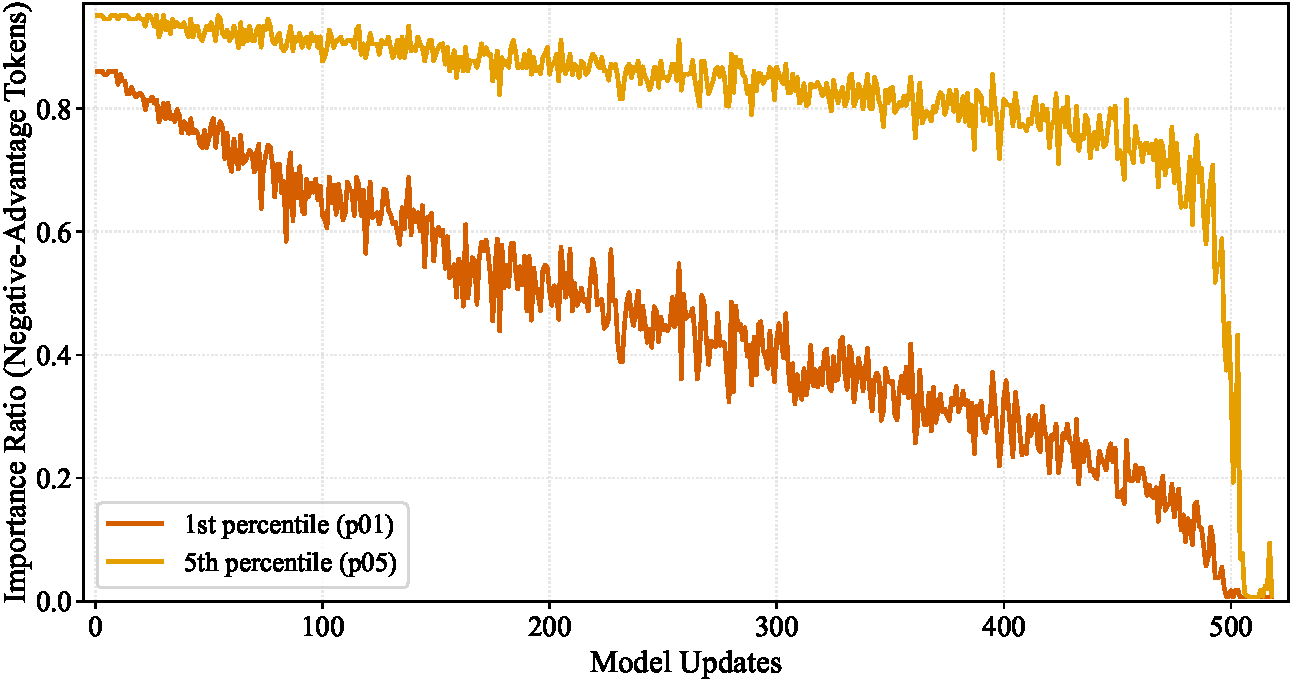
\includegraphics[width=\textwidth]{figures/veto1.pdf}
        \caption{Quantile evolution (p01 and p05) of importance ratios for negative-advantage tokens under high-staleness GRPO with relaxed PPO bounds.
        The left tail of the distribution expands progressively: the p01 quantile first collapses abruptly to values very close to zero, followed shortly by the p05 quantile, indicating a systematic left-tail degeneration rather than isolated outliers.}
        \label{fig:veto1}
    \end{subfigure}
    \hfill
    \begin{subfigure}[t]{0.48\textwidth}
        \centering
        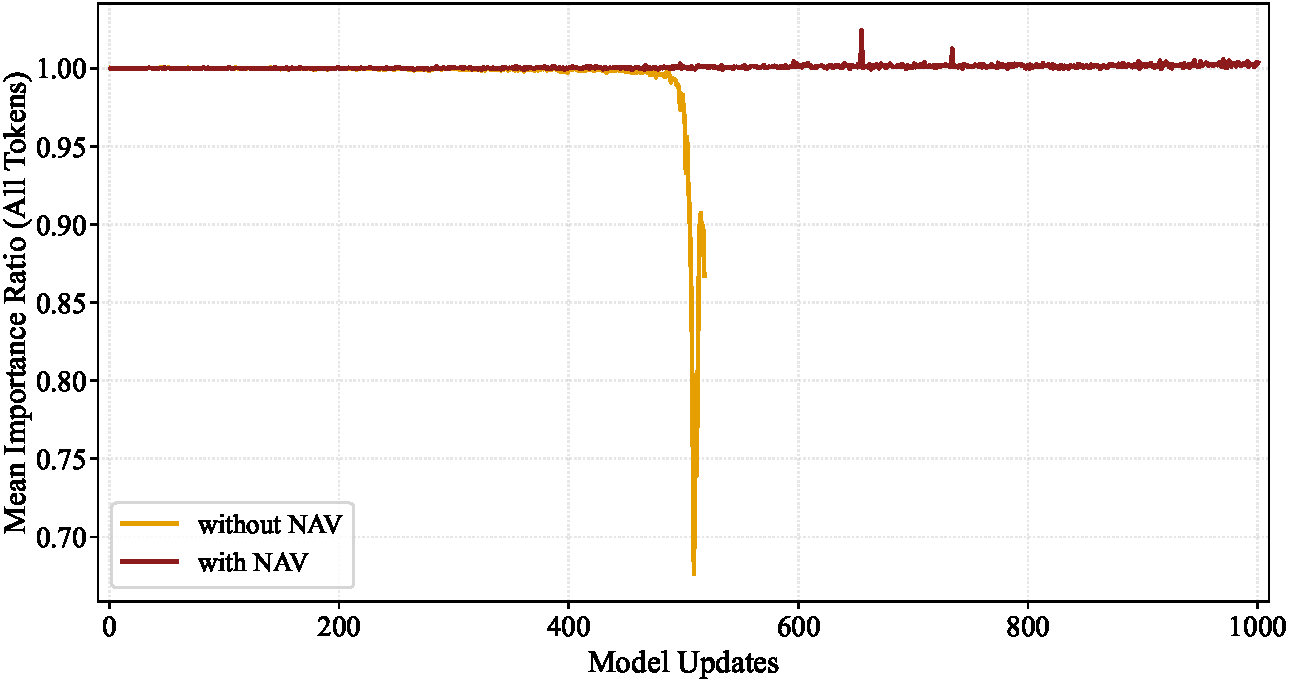
\includegraphics[width=\textwidth]{figures/veto2.pdf}
        \caption{Mean importance ratio over all tokens under high-staleness GRPO with relaxed PPO bounds, with and without negative-advantage veto (NAV).
        As a result of the left-tail expansion indicated in the left panel, the mean importance ratio soon exhibits severe downward oscillations, signaling the emergence of widespread off-support trajectories.}
        \label{fig:veto2}
    \end{subfigure}

    \caption{Training instability of high-staleness GRPO with relaxed PPO bounds $(-\infty, 5)$ on Qwen2.5-Math-7B.
    Evaluation performance collapses at approximately 500 training updates.
    The instability is preceded by a progressive left-tail expansion of negative-advantage importance ratios (left), which is followed shortly by a sharp downward fluctuation of the mean importance ratio (right), indicating large-scale off-support behavior that ultimately destabilizes training.}
    \label{fig:veto}
\end{figure}
